\documentclass[aspectratio=169,11pt]{beamer}
\usepackage[T1]{fontenc}
\usepackage[utf8]{inputenc}
\usepackage[polish]{babel}
\usepackage{booktabs}
\usetheme{default}
\usecolortheme{seahorse}
\setbeamertemplate{navigation symbols}{}
\setbeamertemplate{footline}[frame number]
\graphicspath{{img/}{../results/}}

\title{Inteligentny system monitorowania opinii}
\subtitle{Analiza sentymentu recenzji gier ze Steama}
\author{Eksploracja Danych Tekstowych -- Projekt 1}
\date{2026/2027}

\begin{document}

\begin{frame}
  \titlepage
\end{frame}

\begin{frame}{Cel i wymagania}
  \begin{itemize}
    \item aplikacja pobiera teksty z Internetu (API) i ocenia sentyment: pozytywny / negatywny
    \item dane do predykcji \textbf{muszą} pochodzić z Internetu, trening może być na danych zebranych wcześniej
    \item dane treningowe i do predykcji -- spójne strukturą i charakterem
    \item prosty GUI
  \end{itemize}
  \vspace{1em}
  \textbf{Moje rozwiązanie:} recenzje gier ze Steama (EN), własny model TF-IDF + regresja
  logistyczna, porównanie z gotowym transformerem, GUI w Streamlit.
\end{frame}

\begin{frame}{Dane: Steam Web API}
  \begin{columns}[T]
    \column{0.55\textwidth}
    \begin{itemize}
      \item \texttt{IUserReviewsService/GetAppReviews} -- oficjalne API, bez klucza
      \item stary adres \texttt{/appreviews} wyłączony 22.10.2026 -- trzeba było przejść na nowy
      \item każda recenzja ma etykietę autora: \emph{polecam / nie polecam}
      \item stronicowanie kursorem, przerwy 1\,s, limit żądań, ponawianie przy 429/5xx
    \end{itemize}
    \column{0.42\textwidth}
    \begin{itemize}
      \item \textbf{trening:} 30 gier, po 400 recenzji poz. i neg. $\rightarrow$ 17\,923 po filtrach
      \item podział 70/15/15, ziarno 42
      \item \textbf{predykcja:} inne gry, pobierane na żywo w GUI
    \end{itemize}
  \end{columns}
\end{frame}

\begin{frame}{Czyszczenie tekstu (pułapki z zajęć)}
  \small
  HTML, BBCode, URL $\rightarrow$ \texttt{don't} $\rightarrow$ \texttt{do not} $\rightarrow$ małe litery
  $\rightarrow$ tokeny (słowa, \texttt{2/10}, \texttt{!}, emoji) $\rightarrow$ stopwords \textbf{bez negacji}
  $\rightarrow$ stemming (Porter)
  \vspace{0.4em}

  \centering
  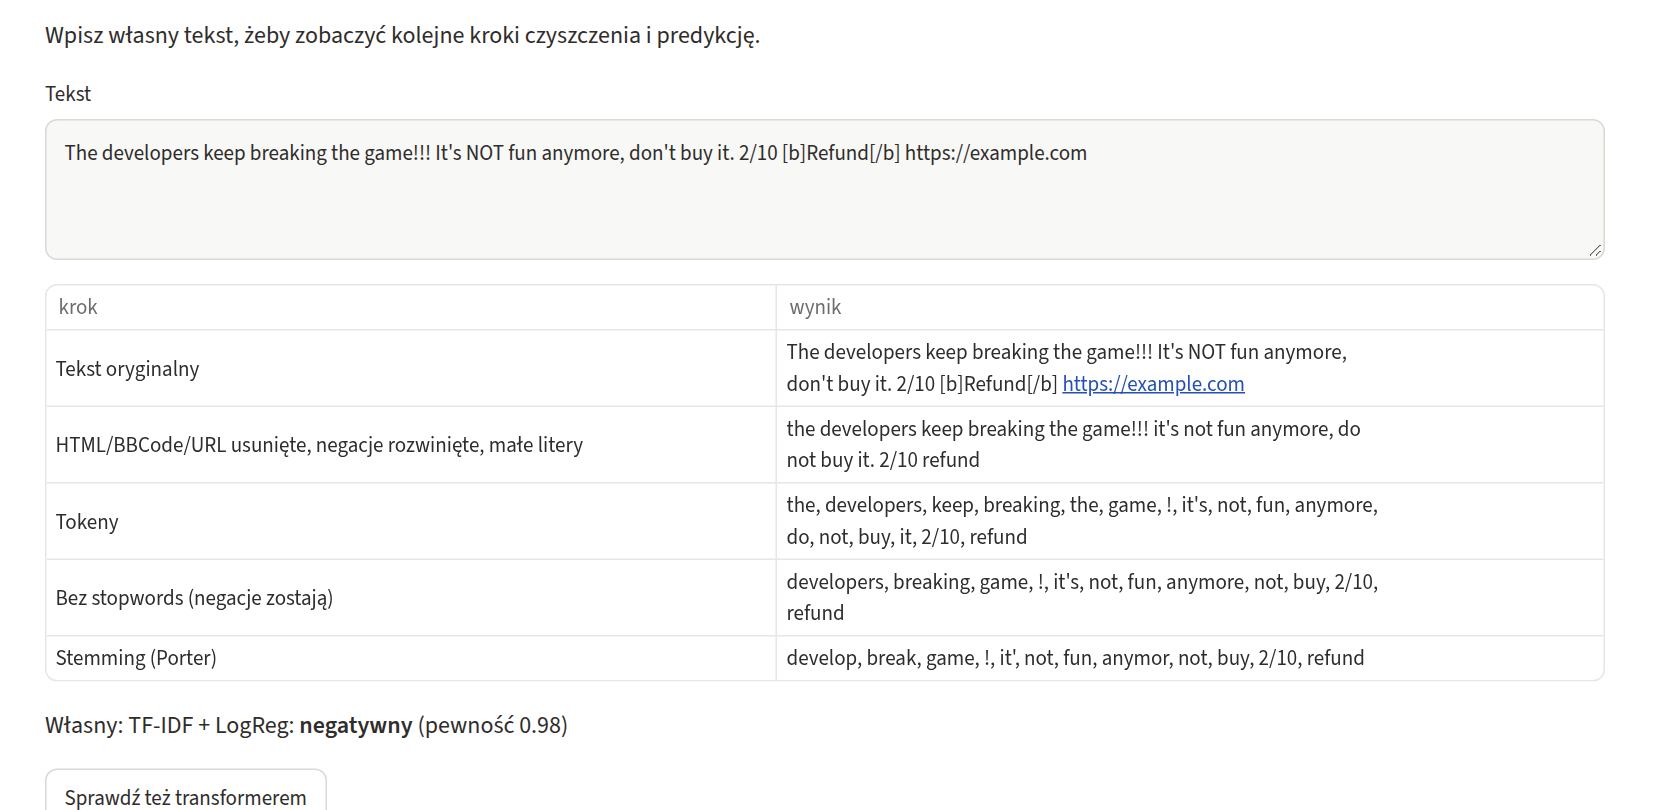
\includegraphics[width=0.86\textwidth]{p1_gui_tekst.png}\\
  \footnotesize Nie usuwam liczb ani wykrzykników -- niosą emocje i oceny (zakładka ,,Pojedynczy tekst'' w GUI).
\end{frame}

\begin{frame}{Stemming czy lematyzacja? Co z negacją?}
  Ten sam model, zmieniam tylko preprocessing (zbiór walidacyjny, \texttt{notebooks/01\_model.ipynb}):
  \vspace{0.5em}
  \begin{center}
  \begin{tabular}{lcc}
    \toprule
    wariant & F1 & czas czyszczenia \\
    \midrule
    bez normalizacji & 0,780 & 0,6 s \\
    \textbf{stemming} & \textbf{0,784} & 3,2 s \\
    lematyzacja (spaCy) & 0,775 & 18,2 s \\
    stemming, stopwords \emph{razem z negacjami} & 0,777 & 3,1 s \\
    \bottomrule
  \end{tabular}
  \end{center}
  \vspace{0.5em}
  \begin{itemize}
    \item różnice małe -- wybieram stemming (najlepszy i kilka razy szybszy)
    \item usunięcie \texttt{not} pogarsza wynik: \emph{,,not good'' $\rightarrow$ ,,good''}
  \end{itemize}
\end{frame}

\begin{frame}{Własny model: TF-IDF + regresja logistyczna}
  \begin{columns}[T]
    \column{0.55\textwidth}
    \begin{itemize}
      \item TF-IDF: unigramy i bigramy (\emph{not recommend}, \emph{not bad})
      \item C dobrane walidacją krzyżową (5 foldów, F1) $\rightarrow$ C = 3
      \item test (2\,689 recenzji): \textbf{F1 = 0,788}, accuracy 0,819, ROC AUC 0,903
      \item największe wagi: \emph{not recommend, refund, unplay, crash} vs.\ \emph{10/10, best, amaz, peak}
      \item model 0,6 MB, 0,2 ms na recenzję
    \end{itemize}
    \column{0.42\textwidth}
    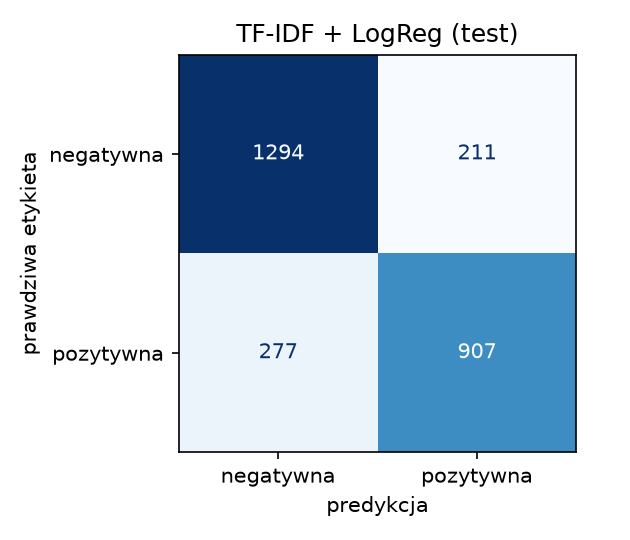
\includegraphics[width=\textwidth]{confusion_matrix.png}
  \end{columns}
\end{frame}

\begin{frame}{Porównanie z transformerem (DistilBERT SST-2)}
  \begin{columns}[T]
    \column{0.58\textwidth}
    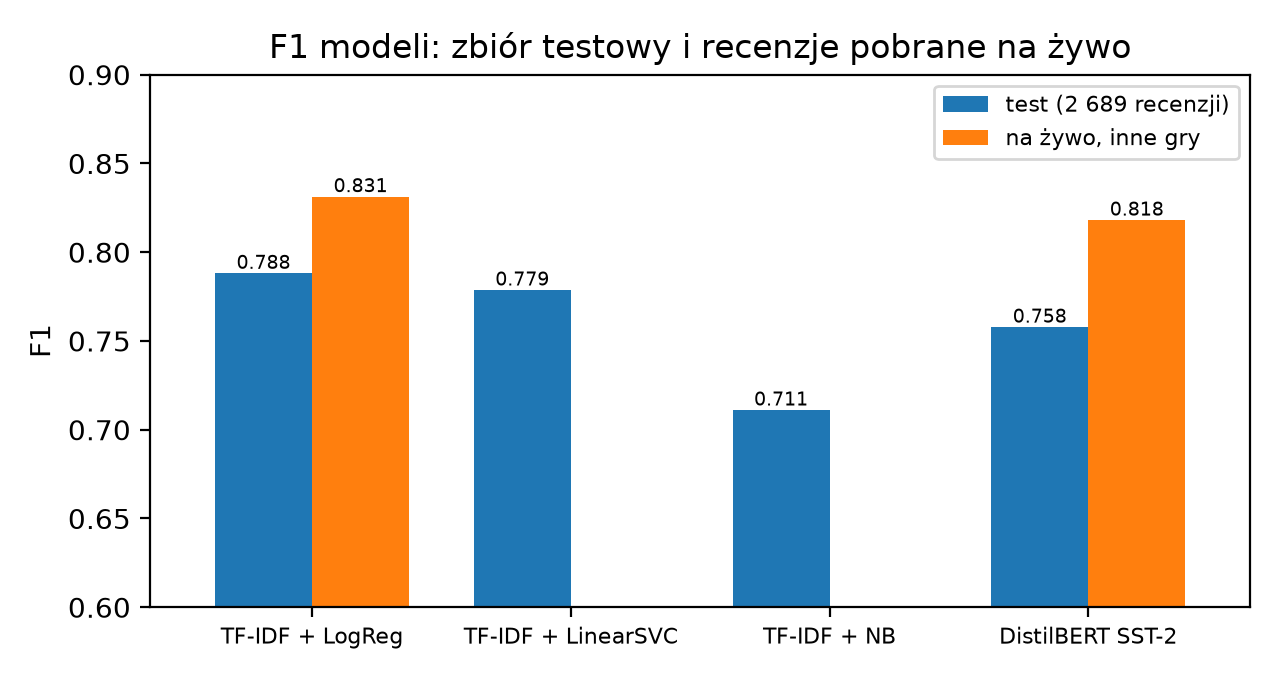
\includegraphics[width=\textwidth]{porownanie_modeli.png}
    \column{0.40\textwidth}
    \small
    \begin{itemize}
      \item gotowy model, dostrojony na recenzjach \emph{filmów}
      \item słabszy na recenzjach gier: nie zna żargonu graczy
      \item ok. 400$\times$ wolniejszy na CPU (92 ms vs 0,2 ms)
      \item ,,na żywo'': 1\,768 recenzji z 9 gier spoza treningu, etykieta autora jako prawda
    \end{itemize}
  \end{columns}
\end{frame}

\begin{frame}{GUI: wyniki dla wybranej gry}
  \centering
  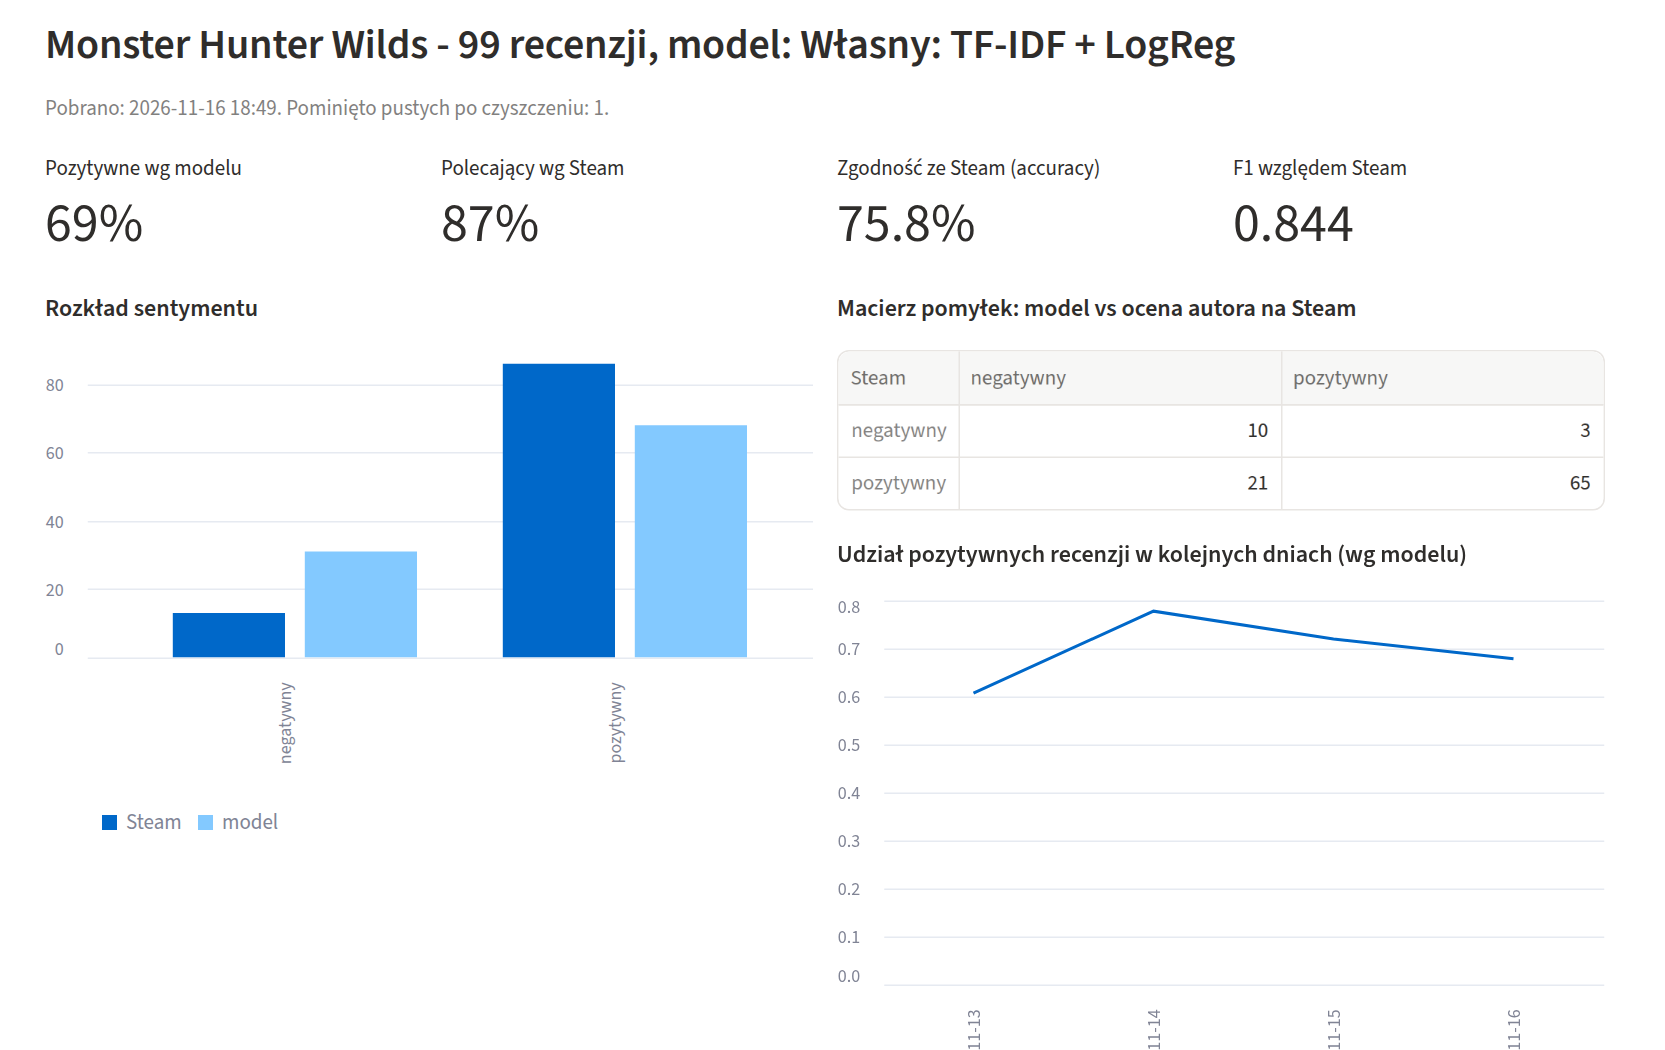
\includegraphics[height=0.80\textheight]{p1_gui_wyniki.png}\\
  \footnotesize wybór gry (lista / nazwa / appid), liczby recenzji i modelu w panelu bocznym
\end{frame}

\begin{frame}{GUI: chmury słów i przykłady}
  \centering
  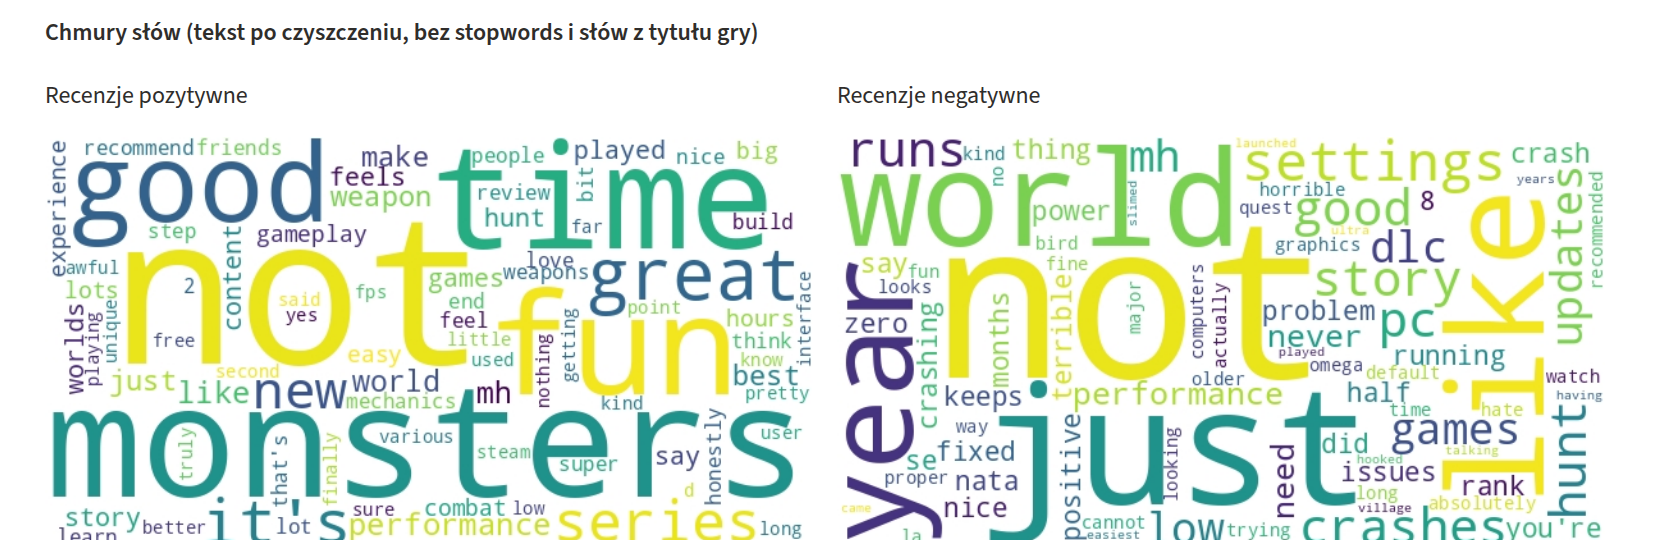
\includegraphics[width=0.85\textwidth]{p1_gui_chmury.png}\\[0.3em]
  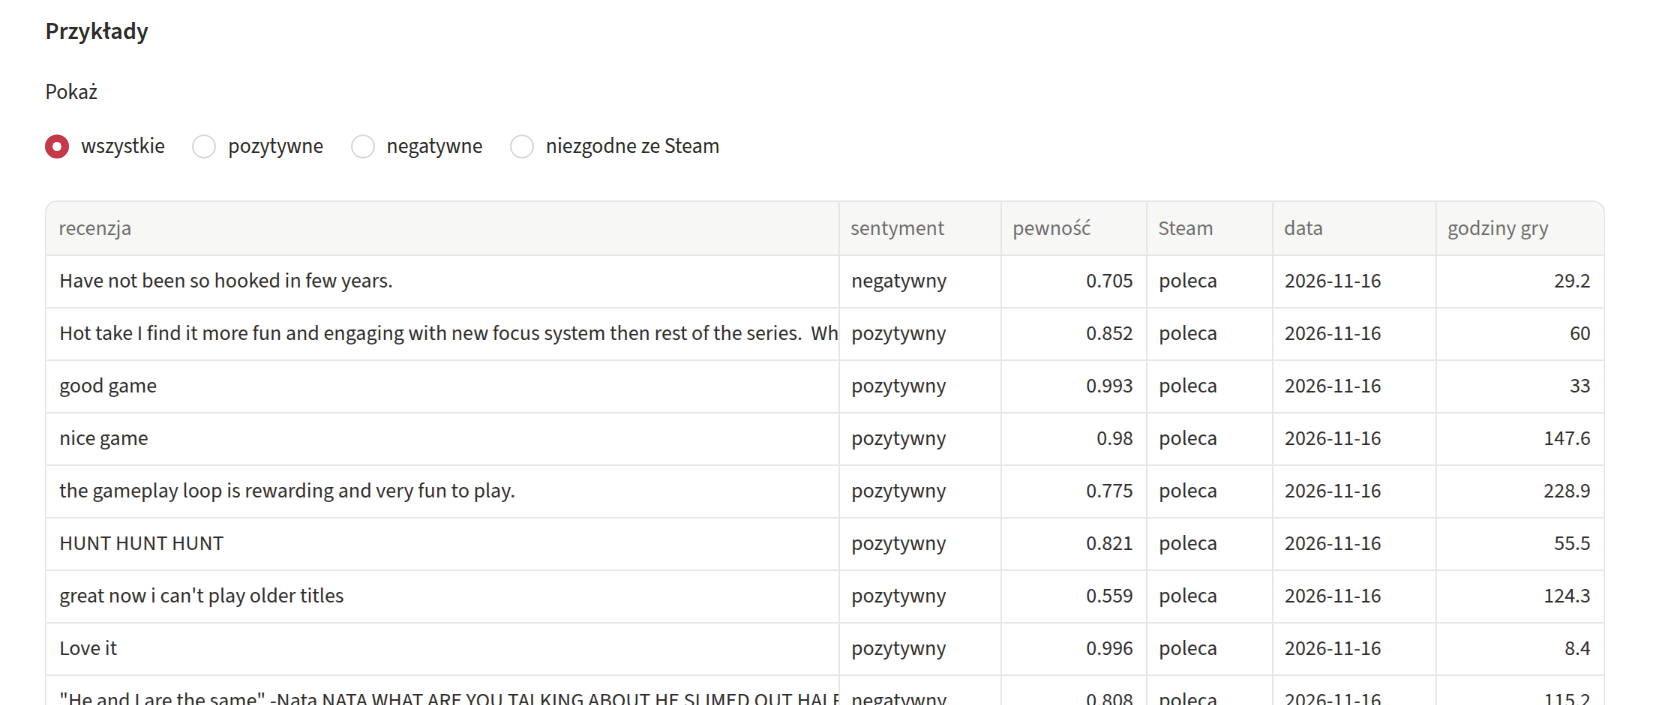
\includegraphics[width=0.85\textwidth]{p1_gui_przyklady.png}
\end{frame}

\begin{frame}{Wnioski i ograniczenia}
  \begin{itemize}
    \item prosty model na danych z tej samej domeny wygrywa z gotowym transformerem z innej domeny
          -- i jest o rzędy wielkości szybszy
    \item warianty preprocessingu różnią się o ok. 0,01 F1; negacji nie wolno usuwać ze stopwords
    \item etykieta ze Steama pozwala zmierzyć trafność także na danych pobranych na żywo
    \item ograniczenia: sarkazm (\emph{,,0/10 would buy again''}), żarty, krytyka wydawcy przy poleceniu gry,
          tylko angielski, bag-of-words nie widzi szyku dalej niż bigram
  \end{itemize}
\end{frame}

\end{document}
